\documentclass[11pt]{article}

\usepackage[margin=1in]{geometry}
\usepackage{amsmath,amssymb,amsthm,mathtools,bm}
\usepackage{booktabs,array}
\usepackage{siunitx}
\usepackage{pgfplots}
\usepackage{algorithm}
\usepackage{algpseudocode}
\usepackage{csquotes}
\usepackage{microtype}
\usepackage{hyperref}
\usepackage[capitalise,noabbrev]{cleveref}
\pgfplotsset{compat=1.18}
\hypersetup{colorlinks=true,linkcolor=black,citecolor=black,urlcolor=blue!50!black}

\theoremstyle{plain}
\newtheorem{theorem}{Theorem}[section]
\newtheorem{lemma}[theorem]{Lemma}
\newtheorem{proposition}[theorem]{Proposition}
\newtheorem{corollary}[theorem]{Corollary}
\theoremstyle{definition}
\newtheorem{definition}[theorem]{Definition}
\theoremstyle{remark}
\newtheorem{remark}[theorem]{Remark}

\newcommand{\Tri}{\operatorname{Tri}}
\newcommand{\BF}{\operatorname{BF}}
\newcommand{\Search}{\operatorname{Search}}
\newcommand{\code}[1]{\texttt{#1}}
\newcommand{\sub}{\sqsubseteq}
\newcommand{\abs}[1]{\left\lvert #1 \right\rvert}
\newcommand{\bigO}[1]{\mathcal{O}\!\left(#1\right)}

\title{Logscope: A Sound Trigram Index\\for Searching Live Log Streams}
\author{Ryan Wetzstein}
\date{November 2026}

\begin{document}
\maketitle

\begin{abstract}
Logscope is a terminal log aggregator that tails files, indexes every line as it
arrives, and answers queries over the live stream. Its index is built on byte
trigrams, with posting lists stored either as delta-varint sequences or as
bitmaps, whichever is smaller, and with per-block timestamp zone maps. The index
may only \emph{prune}: every candidate is verified against the full predicate, so
the result set equals that of a brute-force scan, a property the test suite and
the benchmarks enforce. We formalize the trigram filter and prove it sound,
derive the choice of posting encoding, state the planner's cost model
(rarest-first intersection that stops once verifying is cheaper than decoding,
with a scan fallback for unselective literals), and give the summary algebra
that extracts required literals from a regular expression together with its
soundness argument. On $100$ million lines ($13.4$ GB), a single-hit token is
found in $0.13$ ms at the median, against $3.7$ s for \code{rg -c}. On $10$
million lines, the speedup over the fastest scanner ranges from $2\times$ for a
phrase in $30\%$ of lines to $5{,}880\times$ for a rare prefix.
\end{abstract}

\tableofcontents

\section{Problem and correctness contract}\label{sec:contract}

A log is a sequence of lines $s_0, s_1, \ldots$ whose ids are assigned in
arrival order. Each line is a byte string with an optional timestamp $\tau_i$ and
a multiset of parsed fields $F_i \subseteq K \times V$. Write $\ell \sub s$ when
$\ell$ is a contiguous substring of $s$. A query $Q$ is a predicate built from
the following atoms.
\begin{description}
  \item[Literal $\ell$] $s \models \ell$ if and only if $\ell \sub s$.
  \item[Regex $r$] $s \models r$ if and only if some substring of $s$ lies in
        the language $L(r)$.
  \item[Field $(k, v)$] $s_i \models (k,v)$ if and only if $(k, v) \in F_i$.
  \item[{Time range $[t_0, t_1]$}] $s_i \models [t_0, t_1]$ if and only if
        $t_0 \le \tau_i \le t_1$.
\end{description}
Atoms are combined by conjunction, by \code{OR} groups (disjunctions of
conjunctions) and by \code{NOT}.

\begin{definition}[Brute-force answer]\label{def:bf}
For a query $Q$, let $\BF(Q) \coloneqq \{\, i : s_i \models Q \,\}$, listed in
ascending order and computed by scanning every line.
\end{definition}

The design rests on one rule: the index computes a \emph{candidate set}
$C(Q)$, and the answer is
\begin{equation}\label{eq:search}
  \Search(Q) \coloneqq \{\, i \in C(Q) : s_i \models Q \,\},
\end{equation}
returned in ascending id order. Field terms are the one exception to
verification, because their postings are exact by construction.

\begin{theorem}[Contract]\label{thm:contract}
If $C(Q) \supseteq \BF(Q)$ for every query $Q$ and every reachable index state,
then $\Search(Q) = \BF(Q)$.
\end{theorem}

\begin{proof}
Every element of $\Search(Q)$ satisfies $Q$ by \cref{eq:search}, so
$\Search(Q) \subseteq \BF(Q)$. Conversely, each $i \in \BF(Q)$ lies in $C(Q)$ by
hypothesis and satisfies $Q$, so it passes verification. Both sets are listed in
ascending order, so they are equal as sequences.
\end{proof}

\Cref{thm:contract} turns correctness into one obligation, that the candidate
set is a superset of the answer, and leaves speed to depend on how small that
superset is. The remaining sections discharge the obligation for each kind of
term. A reachable state includes any sequence of inserts, seals, merges,
reopens and retention drops; a model-based property test checks the contract
against a brute-force oracle over such sequences (\cref{sec:eval}).

\section{The trigram filter}\label{sec:trigram}

\subsection{Definitions}

For a byte string $s = b_0 b_1 \cdots b_{n-1}$, the trigram set is
\begin{equation}
  \Tri(s) \coloneqq \{\, b_i b_{i+1} b_{i+2} : 0 \le i \le n - 3 \,\},
\end{equation}
and each trigram is keyed as a $24$-bit integer held in a \code{u32},
\begin{equation}
  \kappa(b_0 b_1 b_2) = 2^{16} b_0 + 2^{8} b_1 + b_2 .
\end{equation}
Working on bytes needs no tokenizer and no assumption about the encoding: a
multi-byte UTF-8 character contributes more trigrams, and invalid UTF-8 costs
nothing extra. The posting list $P(t)$ is the sorted set of ids of lines that
contain trigram $t$.

\subsection{Soundness}

\begin{lemma}[Substring monotonicity]\label{lem:mono}
If $\ell \sub s$, then $\Tri(\ell) \subseteq \Tri(s)$.
\end{lemma}

\begin{proof}
Let $\ell = s[j \mathinner{..} j + \abs{\ell})$. The trigram of $\ell$ at offset
$i$ is the trigram of $s$ at offset $j + i$.
\end{proof}

\begin{proposition}[The literal filter is sound]\label{prop:literal}
For a literal $\ell$ with $\abs{\ell} \ge 3$, define
\begin{equation}\label{eq:literal}
  C(\ell) \coloneqq \bigcap_{t \in \Tri(\ell)} P(t).
\end{equation}
Then $\{\, i : \ell \sub s_i \,\} \subseteq C(\ell)$.
\end{proposition}

\begin{proof}
If $\ell \sub s_i$, then every $t \in \Tri(\ell)$ lies in $\Tri(s_i)$ by
\cref{lem:mono}, so $i \in P(t)$ for each such $t$.
\end{proof}

The converse fails: \code{abcXbcd} contains every trigram of \code{abcd} but not
\code{abcd} itself, which is why candidates are verified with a substring search.
A literal shorter than three bytes has no trigram, so it gives no pruning and is
left to verification.

\paragraph{Case-insensitive search without a second index.} Under ASCII case
folding, each trigram $t$ has at most $2^3 = 8$ case variants $\mathcal{V}(t)$.
The planner replaces $P(t)$ by $\bigcup_{t' \in \mathcal{V}(t)} P(t')$, which is
sound by the argument of \cref{prop:literal} applied to the folded line. Folding
is ASCII-only on purpose, so the variants cover exactly the lines that the
verifier accepts.

\subsection{Disjunction and negation}

For an \code{OR} group $Q = Q_1 \vee \cdots \vee Q_m$, we take
$C(Q) \coloneqq \bigcup_j C(Q_j)$, a superset of the answer because each
$C(Q_j)$ is one. If any branch cannot prune, that is, $C(Q_j)$ is every line,
then neither can the group. For $\neg Q'$, the index can prove that a line
\emph{contains} a trigram but never that a line \emph{lacks} a string, so
negation is verify-only: it removes lines after the fact and never shrinks $C$.

\section{Storage}\label{sec:storage}

\subsection{Segments}

New lines go to a mutable \emph{active} segment, a hash map from trigram key to
a growing list of segment-local ids. At $200{,}000$ lines (the default) it is
sealed into an immutable, memory-mapped file. Segments cover consecutive id
ranges $[\beta_j, \beta_j + n_j)$, so concatenating the per-segment sorted results
in segment order yields globally sorted ids with no merge step.

\subsection{Posting encoding}

A sealed posting list $L = (x_1 < x_2 < \cdots < x_m)$ over a segment of $n$
lines is written in one of two forms.

\paragraph{Delta and varint.} The gaps $g_1 = x_1$ and $g_j = x_j - x_{j-1}$ are
written as LEB128 varints, seven payload bits per byte with the high bit set on
every byte but the last. A gap $g$ therefore costs
\begin{equation}
  \nu(g) = \max\!\left(1, \left\lceil \frac{\lfloor \log_2 g \rfloor + 1}{7} \right\rceil\right)
  \text{ bytes}, \qquad
  \abs{L}_{\text{var}} = \sum_{j=1}^{m} \nu(g_j).
\end{equation}

\paragraph{Bitmap.} One bit per line gives
$\abs{L}_{\text{bit}} = \lceil n / 8 \rceil$ bytes. The encoder writes the bitmap
exactly when $\abs{L}_{\text{bit}} < \abs{L}_{\text{var}}$ and flags the choice
in the top bit of the stored count.

\begin{proposition}[Dense lists become bitmaps]\label{prop:bitmap}
Every list with $m > \lceil n/8 \rceil$ postings, that is, with density
$\rho \coloneqq m/n$ above about $1/8$, is stored as a bitmap.
\end{proposition}

\begin{proof}
Each gap costs at least one byte, so $\abs{L}_{\text{var}} \ge m > \lceil n/8
\rceil = \abs{L}_{\text{bit}}$.
\end{proof}

For a list spread evenly at density $\rho$, the gaps are close to $1/\rho$, so
the varint form costs about $m\,\nu(1/\rho)$ bytes. Each byte covers a factor of
$2^7 = 128$ in gap size, so the cost per posting steps from one to two bytes near
$\rho = 1/128$ and from two to three near $\rho = 1/16{,}384$. Common trigrams in
log text, such as \code{=er}, fall in the bitmap regime, where intersection is a
bit test per candidate instead of a decode.

\subsection{Timestamp zone maps}

Lines are grouped in blocks of $B = 1024$. For block $b$ the segment stores
$m_b \coloneqq \min_{i \in b}\tau_i$ and $M_b \coloneqq \max_{i \in b}\tau_i$.
For a time range $[t_0, t_1]$, block $b$ is skipped whenever
\begin{equation}
  [m_b, M_b] \cap [t_0, t_1] = \varnothing, \quad\text{that is,}\quad M_b < t_0 \;\text{ or }\; m_b > t_1 .
\end{equation}
The skip is sound because no line in such a block can satisfy the range. A time
query costs $\bigO{n/B}$ comparisons plus the work in surviving blocks; on mostly
ordered logs only the blocks at the two ends of the range need line-level checks.

\section{Query planning}\label{sec:planning}

\subsection{Cost model}

The planner prices work at one unit per decoded posting and charges
$c_v = 16$ units per verified candidate (\code{VERIFY\_COST}). Each term $t$ (a
trigram, a union of case variants, a regex clause, a field or a time range) has a
count $\abs{P(t)}$ known from the dictionary without decoding.
\Cref{alg:plan} intersects the terms.

\begin{algorithm}[htbp]
\caption{Rarest-first intersection with early stop}\label{alg:plan}
\begin{algorithmic}[1]
\State sort the terms so that $\abs{P(t_1)} \le \abs{P(t_2)} \le \cdots \le \abs{P(t_k)}$
\State $A \gets \bot$
\For{$j = 1, \ldots, k$}
  \If{$A \ne \bot$ \textbf{and} $t_j$ is optional \textbf{and} $c_v \abs{A} < \abs{P(t_j)}$}
    \State \textbf{continue} \Comment{verifying $A$ costs less than decoding $P(t_j)$}
  \EndIf
  \State $A \gets P(t_j)$ \textbf{if} $A = \bot$ \textbf{else} $A \cap P(t_j)$
  \If{$A = \varnothing$} \Return no matches \EndIf
\EndFor
\State \Return candidates $A$, to be verified
\end{algorithmic}
\end{algorithm}

\begin{proposition}[Skipping is safe and pays]\label{prop:skip}
Skipping an optional term never changes the answer. When the skip condition
holds, including the term costs more than the verification work it could save.
\end{proposition}

\begin{proof}
Each term's postings form a superset of the lines satisfying that term, so the
intersection of any subset of terms is a superset of $\BF(Q)$, and
\cref{thm:contract} applies. For the cost, finishing without $t_j$ costs at most
$c_v \abs{A}$ for verification, whereas including $t_j$ costs at least
$\abs{P(t_j)}$ to decode. Under the condition $c_v \abs{A} < \abs{P(t_j)}$ the
second exceeds the first even if $t_j$ removed every candidate.
\end{proof}

Field terms are \emph{mandatory}: verification cannot re-check them, since their
postings define a field match, so they are never skipped. Sorting by
$\abs{P(t)}$ keeps intermediate sets small, because each intersection is bounded
by its smaller operand.

\subsection{Scan fallback}

For a literal $\ell$ over a segment of $n$ lines, let
$\mu(\ell) \coloneqq \min_{t \in \Tri(\ell)} \abs{P(t)}$. If
\begin{equation}\label{eq:scan}
  D\,\mu(\ell) \ge n, \qquad D = 8 \;(\code{SCAN\_DIVISOR}),
\end{equation}
then no trigram of $\ell$ excludes more than $7/8$ of the lines, and one
\code{memchr::memmem} pass over the segment's concatenated text costs less than
any intersection. The planner then scans instead of using the index.

\subsection{Parallelism}

A list of $n$ items is split across threads only when $n \ge 16{,}384$, into
$\operatorname{clamp}(T, 1, \lfloor n / 4096 \rfloor)$ contiguous parts for $T$
available threads, so that each part keeps at least $4{,}096$ items. The parts'
results are concatenated in order and remain sorted.

\section{Regex literal extraction}\label{sec:regex}

To prune for a regex $r$, Logscope derives a conjunction of \emph{clauses}, each
a set of alternative strings, such that every match contains at least one
alternative of every clause.

\begin{definition}[Node summary]\label{def:summary}
For a regex node $h$, a summary is a pair $(E, \mathcal{C})$ in which $E$ is
either a finite set of strings or $\bot$, and $\mathcal{C}$ is a set of clauses.
The summary is \emph{sound} for $h$ if every $w \in L(h)$ satisfies both of the
following:
\begin{enumerate}
  \item if $E \ne \bot$, then $w \in E$;
  \item for every clause $X \in \mathcal{C}$ there is some $x \in X$ with $x \sub w$.
\end{enumerate}
\end{definition}

Summaries are computed bottom-up over the regex syntax tree. Two bounds keep the
sets small: $\abs{E} \le 16$, and every string in $E$ is at most $48$ bytes long.
To \emph{flush} an exact set $E$ means to turn it into the clause $E$, which says
that every match contains one of its strings; a flushed clause with an
alternative shorter than three bytes is dropped, since it has no trigram to look
up. The rules are as follows.
\begin{description}
  \item[Literal $c$] $(\{c\}, \varnothing)$.
  \item[Class] $(\text{its members}, \varnothing)$ when the class has at most
        $8$ code points, and $(\bot, \varnothing)$ otherwise.
  \item[Concatenation $h_1 h_2 \cdots$] The running exact set is extended by
        the cross product $E \cdot E_j \coloneqq \{\, xy : x \in E, y \in E_j \,\}$
        while it stays within the bounds. When a part is not exact, or the product
        would exceed the bounds, the running set is flushed and restarted, and the
        result's $E$ becomes $\bot$. Child clauses are kept.
  \item[Alternation $h_1 \mid \cdots \mid h_m$] If every branch is exact and the
        union fits the bounds, $(\bigcup_j E_j, \varnothing)$. Otherwise, from
        each branch the clause whose shortest alternative is longest is chosen,
        and the chosen clauses are joined into one clause,
        $(\bot, \{X_1 \cup \cdots \cup X_m\})$. If some branch has no clause, the
        result is $(\bot, \varnothing)$.
  \item[Optional $h?$] $(E \cup \{\varepsilon\}, \varnothing)$ when $h$ is exact
        and the set fits, and $(\bot, \varnothing)$ otherwise.
  \item[Star $h*$, or any repetition with minimum $0$] $(\bot, \varnothing)$.
  \item[Repetition with minimum $m \ge 1$] $(\bot, \mathcal{C} \cup \{E\})$,
        with $E$ flushed into a clause.
\end{description}

\begin{lemma}[Rules preserve soundness]\label{lem:rules}
If the children's summaries are sound, the parent's summary is sound.
Consequently, by structural induction, the clauses computed for any regex are
satisfied by every match.
\end{lemma}

\begin{proof}[Proof sketch]
Literals and small classes are exact by definition. For a concatenation, a match
is $w = w_1 w_2 \cdots$ with $w_j \in L(h_j)$; while every part is exact, $w$ lies
in the cross product, and after a flush the flushed set still occurs as a
contiguous substring of $w$, so its clause holds. Child clauses hold for $w_j$
and hence for $w$, because a substring of $w_j$ is a substring of $w$. For an
alternation, a match takes exactly one branch $j$, so it contains some element
of that branch's chosen clause $X_j$, and therefore some element of the union.
An optional node matches either $\varepsilon$ or a match of $h$; a repetition with
minimum $m \ge 1$ contains at least one match of $h$ as a substring; a repetition
with minimum $0$ asserts nothing. Dropping a clause and replacing \enquote{$w \in
E$} by \enquote{$w$ contains some $x \in E$} both weaken a sound summary, so
soundness is kept.
\end{proof}

The candidate set for $r$ is then
\begin{equation}\label{eq:regex}
  C(r) \coloneqq \bigcap_{X \in \mathcal{C}} \; \bigcup_{x \in X} C(x),
\end{equation}
a superset of the lines matching $r$ by \cref{lem:rules,prop:literal}. For
example, \code{foo(bar|baz)} yields the single clause
$\{\code{foobar}, \code{foobaz}\}$, and \code{conn(ection)?\ reset} yields
\[
  \{\code{conn reset},\; \code{connection reset}\}.
\]
A randomized property test generates regexes and texts and checks the statement
of \cref{lem:rules} directly.

\section{Segment merging}\label{sec:merge}

Once there are more than $M = 12$ sealed segments $S_1, \ldots, S_k$ with byte
sizes $b_1, \ldots, b_k$, the engine merges one contiguous run of neighbours.
Merging $r$ segments into one leaves $k - r + 1$ segments, so reaching $M$
requires $r = k - M + 1$. Among the $k - r + 1 = M$ windows of that length, the
engine picks the one that rewrites the fewest bytes, subject to a cap
$\bar{b} = 512$ MiB:
\begin{equation}
  j^\star = \arg\min_{1 \le j \le M} \; \sum_{i=j}^{j+r-1} b_i
  \quad\text{subject to}\quad \sum_{i=j}^{j+r-1} b_i \le \bar{b}.
\end{equation}
Contiguity preserves the id-range order of segments, and the cheapest window
tends to merge recent small segments, which gives a tiered structure without
rewriting the whole index. The merged file is written before its inputs are
deleted, so a crash at any point leaves either the inputs or a covering output,
and recovery keeps the covering one.

\section{Live queries}\label{sec:live}

A standing query $Q$ is checked against each inserted batch as it enters the
index, so a live view costs $\bigO{\text{new lines}}$ and never re-searches. A
relative window such as \code{last 5m} stays symbolic until it is resolved at
time $t_{\text{now}}$ to $[t_{\text{now}} - 300\,\text{s}, t_{\text{now}}]$, and the
interface re-resolves it every $2$ s so that the window slides. The ingest batcher
flushes at $1{,}024$ records or $50$ ms after the first record, whichever comes
first, which bounds the delay that a quiet source adds to $50$ ms.

\section{Evaluation}\label{sec:eval}

The corpus is synthetic logfmt, about $130$ bytes per line, with a rare
\code{token=} field every $100{,}003$ lines and log time advancing $1$ ms per ten
lines. Every method must return identical match counts for every query, or the
run aborts. \Cref{tab:10m} gives the fully warm results at $10$ million lines and
\cref{fig:speedup} the speedups.

\begin{table}[htbp]
\centering
\caption{At $10$M lines ($1.33$ GB), selective queries finish in microseconds
to milliseconds while every scanner needs tens to hundreds of milliseconds.
Latencies are medians; the scan is an in-process \code{memchr}/\code{regex}
pass over the memory-mapped file, the fair lower bound for a scanner. Speedup is
against the fastest of scan, \code{grep} and \code{rg}.}
\label{tab:10m}
\small
\begin{tabular}{l r S[table-format=2.3] S[table-format=3.1] S[table-format=3.1] r}
\toprule
Query & Matches & {Logscope (ms)} & {Scan (ms)} & {\code{rg} (ms)} & Speedup \\
\midrule
unique token           & 1         & 0.013  & 47.4  & 326.2 & $3765\times$ \\
rare token prefix      & 100       & 0.007  & 40.6  & 318.5 & $5880\times$ \\
one second of time     & 10{,}000  & 0.068  & 41.5  & 319.5 & $614\times$ \\
field filter           & 167{,}032 & 0.974  & 60.3  & 353.3 & $62\times$ \\
field and literal      & 166{,}145 & 3.880  & 630.3 & 474.1 & $122\times$ \\
phrase, 1.7\% of lines & 166{,}727 & 4.809  & 44.1  & 341.9 & $9\times$ \\
regex with literals    & 332{,}761 & 9.988  & 531.6 & 408.8 & $41\times$ \\
common phrase, 30\%    & 1{,}249{,}824 & 36.322 & 54.9 & 356.3 & $2\times$ \\
regex, weak literals   & 889{,}853 & 72.008 & 433.7 & 710.3 & $6\times$ \\
\bottomrule
\end{tabular}
\end{table}

\begin{figure}[htbp]
\centering
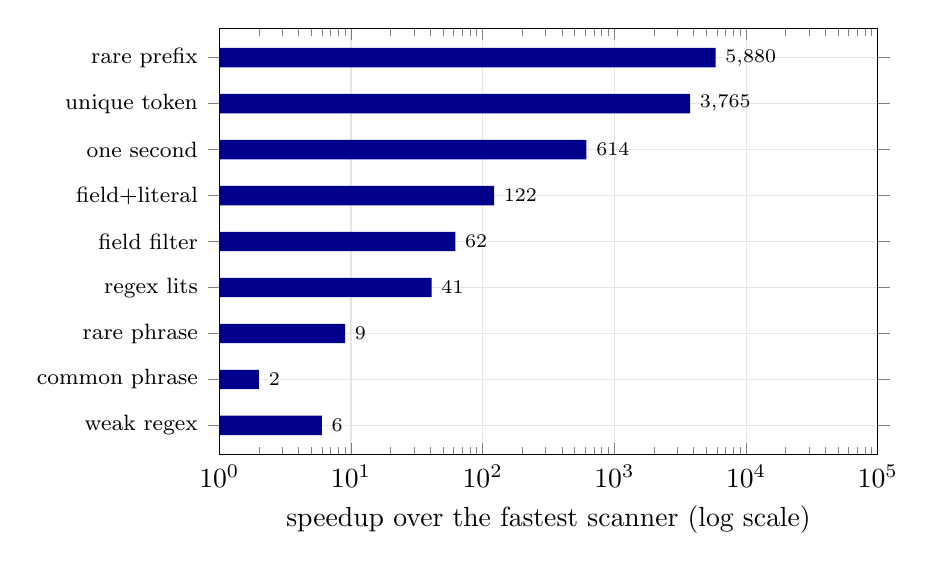
\begin{tikzpicture}
\begin{axis}[
  xbar, width=0.82\textwidth, height=7cm,
  xmode=log, log origin=infty,
  xlabel={speedup over the fastest scanner (log scale)},
  symbolic y coords={weak regex, common phrase, rare phrase, regex lits, field filter, field+literal, one second, unique token, rare prefix},
  ytick=data, y tick label style={font=\footnotesize}, enlarge y limits=0.08,
  xmin=1, xmax=100000, bar width=7pt,
  nodes near coords, nodes near coords align={horizontal}, nodes near coords style={font=\scriptsize},
  point meta=rawx, every node near coord/.append style={/pgf/number format/fixed, /pgf/number format/precision=0},
  grid=major, grid style={gray!20}]
\addplot[fill=blue!55!black, draw=none] coordinates {
  (6,weak regex) (2,common phrase) (9,rare phrase) (41,regex lits) (62,field filter)
  (122,field+literal) (614,one second) (3765,unique token) (5880,rare prefix)};
\end{axis}
\end{tikzpicture}
\caption{Speedup grows with selectivity, from $2\times$ for a phrase in $30\%$ of
lines to $5{,}880\times$ for a rare prefix. Unselective queries are bound by
memory bandwidth either way, and the scan fallback of \cref{eq:scan} keeps them
from being slower than a scan.}
\label{fig:speedup}
\end{figure}

\paragraph{Scale.} On $100$M lines ($13.4$ GB), a single-hit token takes
$0.13$ ms at the median, against $3{,}722$ ms for \code{rg -c} and $7{,}753$ ms for
\code{grep -c}. At that size, $13$ GB of text plus $24$ GB of index exceed the test
machine's free memory, so those runs include cold page-cache reads.

\paragraph{Cost.} At $10$M lines the index is $182\%$ of the raw data, of which
$100\%$ is the stored copy of the text, kept so that results survive log
rotation; the trigram, field and time structures account for $83\%$. Indexing
ran at about $1.32$M lines per second ($7.6$ s for $10$M lines).

\paragraph{Correctness testing.} Beyond the benchmark's count check, a
model-based property test drives random inserts, seals, merges, reopens and
searches against the brute-force oracle of \cref{def:bf}, over a small alphabet
with multi-byte characters that forces shared trigrams and long lists. Planner
tests force every path by running each query with $c_v \in \{0, \infty\}$ and
with the scan divisor at both extremes.

\section{Limitations}\label{sec:limits}

\begin{description}
  \item[Unselective queries] When the answer is a large fraction of the log, it
        must be produced line by line, and the index offers little over a scan
        ($2\times$ at $30\%$ selectivity).
  \item[Weak regex literals] A regex whose required literals occur in every
        line has nothing to prune with.
  \item[No ranking] Trigrams support substring and regex search with no
        tokenizer, but results are chronological, not scored.
  \item[One corpus, one machine] The benchmarks use a single synthetic logfmt
        corpus; real logs with more varied vocabularies will have different
        trigram densities.
\end{description}

\section*{Preparation}

This paper was drafted with an AI assistant (Claude) from the project's source
code, design notes and benchmark results, and checked against them; the author
is responsible for its content. \Cref{app:provenance} lists the source of every
number.

\section*{License}

\copyright\ 2026 Ryan Wetzstein. This paper is licensed under the Creative
Commons Attribution 4.0 International License (CC BY 4.0,
\url{https://creativecommons.org/licenses/by/4.0/}). The license covers the
text and figures of this paper, not the Logscope software, whose rights remain
reserved.

\appendix
\section{Provenance of numbers}\label{app:provenance}

\begin{table}[htbp]
\centering
\caption{Where each reported number comes from. Paths are relative to the
\code{logscope} repository at commit \code{b65f986}; the planner and format
sources are under \code{crates/ls-index/src/}.}
\label{tab:provenance}
\small
\begin{tabular}{>{\raggedright\arraybackslash}p{0.42\textwidth} >{\raggedright\arraybackslash}p{0.52\textwidth}}
\toprule
Number & Source \\
\midrule
Trigram key, bitmap rule, varint coding, block size $B = 1024$ & \code{format.rs} \\
$c_v = 16$, $D = 8$, parallel threshold $16{,}384$ & \code{search.rs} \\
Regex bounds ($16$ strings, $48$ bytes, $8$ code points) and rules & \code{regex\_lits.rs} \\
$M = 12$ segments, merge cap $512$ MiB & \code{index.rs}, \code{docs/DESIGN.md} \\
Seal size $200{,}000$ & \code{crates/ls-tui/src/settings.rs} \\
Batcher $1{,}024$ records or $50$ ms; $2$ s window refresh & \code{docs/DESIGN.md} \\
$10$M latencies, counts, index ratio, build time & \code{bench/results/10M.md} \\
$100$M latencies and sizes & \code{README.md} \\
Corpus description & \code{bench/README.md} \\
\bottomrule
\end{tabular}
\end{table}

\paragraph{Not confirmed.} The $100$M figures come from the README; the
matching benchmark results file was not re-read. The README quotes the index
as $183\%$
of the raw data, while the $10$M results give $182\%$; this paper uses the $10$M
value. No benchmark was re-run for this paper.

\end{document}
